\documentclass[10pt]{article}

\RequirePackage{nybohansenPreamble}

\usepackage[draft]{fixme}
\newcommand{\authorName}{Mads Ohm Larsen and Kasper Nybo Hansen}
\newcommand{\authorEmail}{\{omega, nybo\}@diku.dk}
\newcommand{\titleName}{Project 2}
\newcommand{\courseName}{Advanced Algorithms 2011}

\author{\authorName \\\texttt{\small{\authorEmail}}}
\title{\textsc{\titleName \\ \courseName}}
\makeindex

\begin{document}
\maketitle    

\section*{Question 1.1} % (fold)
\label{sec:question_1_1}
\paragraph{Part A} % (fold)
\label{par:part_a}

We are given a complete undirected graph $G = (V,E)$, with non-negative weights $d_{ij}$, and a viewing distance $d$. 

Find the shortest cycle starting and ending in a node $v_0 \in V$, where each vertex $v \in V$ is `visited'. Let the cycle consist of the path $p = \{v_0, v_1,v_2,...,v_n, v_0\}$, then the edge, $e_{ij}$, between two adjacent vertices $v_i$ $v_j$ in the path must meet $d_{ij}\leq d$. 

Transforming the above definition into a decision problem would, instead of finding the shortest cycle, be a question of, is there a cycle of some length $l$, which satisfy the above.


\fxnote{Give the corrosponding language?}

% paragraph part_a (end)

\paragraph{Part B} % (fold)
\label{par:part_b}

% paragraph part_b (end)
% section question_1_1 (end)

\section*{Question 1.2} % (fold)
\label{sec:question_1_2}
% Tror måske det kan gøres således:
%    A - B
%     \ /
%      C
% Den korteste TCP cycle er A (eller B eller C), men det mindste 1-tree indeholder alle knuderne

\begin{figure}
	\centering
	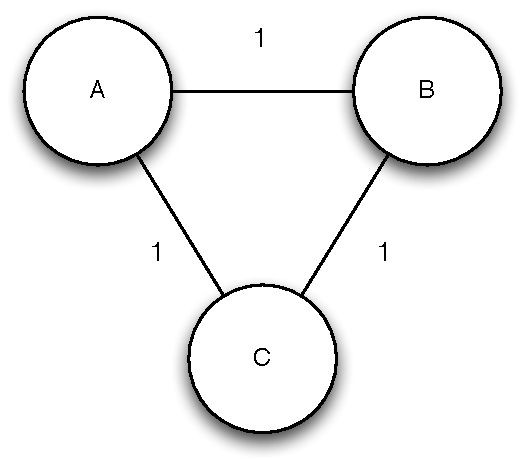
\includegraphics[width=0.4\textwidth]{figures/unicycle.pdf}
	\caption{A graph where the smallest 1-tree is larger than the optimal TCP cycle. $d<1$}
	\label{unicycle}
\end{figure}
In figure \ref{unicycle} we have depicted a set of points $A$, $B$ and $C$, in which the smallest 1-tree, $A-B-C$ is larger than the optimal TCP cycle, which can be one of the three points.
The $d$ value is in this instance less than one.
% section question_1_2 (end)

\section*{Question 1.3} % (fold)
\label{sec:question_1_3}

% section question_1_3 (end)

\section*{Question 1.4} % (fold)
\label{sec:question_1_4}

% section question_1_4 (end)

\section*{Question 2.1} % (fold)
\label{sec:question_2_1}

% section question_2_1 (end)

\section*{Question 2.2} % (fold)
\label{sec:question_2_2}

% section question_2_2 (end)

%\section*{Question 2.3} % (fold)
%\label{sec:question_2_3}
% Optional
% section question_2_3 (end)


%\bibliographystyle{abbrv}
%\bibliography{bibliography}

\end{document}                      



